\documentclass{scrartcl}
\usepackage[polish]{babel}
\usepackage[utf8]{inputenc}
\usepackage[OT4]{fontenc}
\usepackage{url}
\usepackage{amsmath}
\usepackage{amsfonts}
\usepackage{graphicx}
\usepackage{chngpage}
\usepackage{caption}
\usepackage{subcaption}

\title{Sztuczna inteligencja DAO}
\date{\today}
\author{Tomasz Boczkowski\\ 88189 \and Paweł Lampe\\ 99277}

\begin{document}

\thispagestyle{empty} %bez numeru strony

\begin{center}
{\large{Projekt z laboratorium:\\
Sztucznej Inteligencji na kierunku Informatyka }}

\vspace{3ex}

Implementacja algorytmów sztucznej inteligencji grających w DAO.

\vspace{3ex}
{\footnotesize Poznań,\today}

\end{center}


\vspace{10ex}


\vspace{5ex}

Autorzy:
\begin{tabular}{lllr}
\textbf{Tomasz Boczkowski} & 88189 & I5.1 & tomasz.boczkowski@onet.pl \\
\textbf{Paweł Lampe} & 99277 & I5.1 & pawel.lampe@poczta.fm \\
\end{tabular}

\vspace{5ex}



\newpage



\section{Opis gry}

Lorem ipsum

\section{Implementacja}

\subsection{Reprezentacja stanu gry}

Stan gry jest reprezentowany na trzy sposoby. Są one wymienione w
poniższych punktach.

\subsubsection{Podstawowa reprezentacja macierzowa}

\subsubsection{Reprezentacja krótka}

TODO: Zamienić biały -> czerwony, czarny->niebieski

Reprezentacja krótka zawiera pełną informację o stanie gry zawartą
w 32--bitowej liczbie całkowitej bez znaku. Jest ona stosowana przy
wykrywaniu cykli.

Stan każdego z 16 pól jest reprezentowany za pomocą dwóch
bitów:
\begin{itemize}
\item $(00)_B$ reprezentuje pole puste
\item $(01)_B$ reprezentuje pole zajęte przez pionek gracza aktualnie
  wykonującego ruch
\item $(10)_B$ reprezentuje pole zajęte przez pionek gracza
  oczekującego na ruch przeciwnika
\item $(11)_B$ stan zakazany, przydatny przy rozpoznawaniu kolorów
  graczy.
\end{itemize}

Reprezentacje stanów pól są konkantenowane zgodnie z kolejnością pól,
przedstawioną na rysunku \ref{fig:field_order}. Tworzą one 32-bitową
liczbę. Jeżeli gracz aktualnie wykonujący ruch ma kolor biały,
utworzona liczba jest reprezentacją krótką stanu gry. Jeżeli kolorem
gracza wykoującego ruch jest czarny, reprezentacja krótka powstaje 
poprzez zanegowanie bitowe utworzonej przez konkatenację liczby.

\begin{figure}[h]
  \centering
  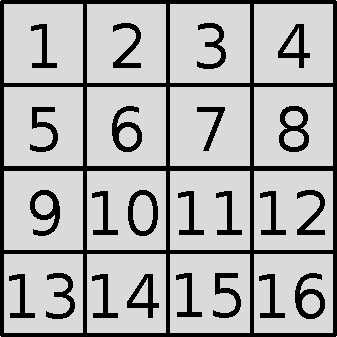
\includegraphics{data/field_order.pdf}
  \caption{Kolejność pól przy obliczaniu reprezentacji krótkiej}
  \label{fig:field_order}
\end{figure}

Kolor gracza wykonującego ruch można określić, wyszukując w
reprezentacji stanu gry sekwencji $(11)_B$. Jest ona obecna wtedy i
tylko wtedy, gdy gracz wykonujący ruch posiada pionki czarne.

TODO: Ująć jakoś, że $(11)_B$ nie jest dowolną sekwencją, lecz jednym
z 16 2--bitowych kawałków.

\subsubsection{Reprezentacja krótka niezmienna względem odbić,
  obrotów i kolorów}
Jest to wariant reprezentacji krótkiej, nie zawierający informacji 
o kolorach pionów. Jest on obliczany w sposób, zapewniający 
niezmienniczość względem obrotów planszy i odbić lustrzanych w pionie
i poziomie. 

Plansze na rysunku \ref{fig:field_order2} zawierają numery pól na
planszy poddanej transformacjom. Dla każdej z 8 transformacji i
określonej przez nią kolejności pól, jest obliczana reprezentacja 
krótka (bez negowania). Spośród obliczonych 8 reprezentacji, 
jest wybierana ta, która stanowi najmniejszą liczbę.

\begin{figure}[h]
  \centering
  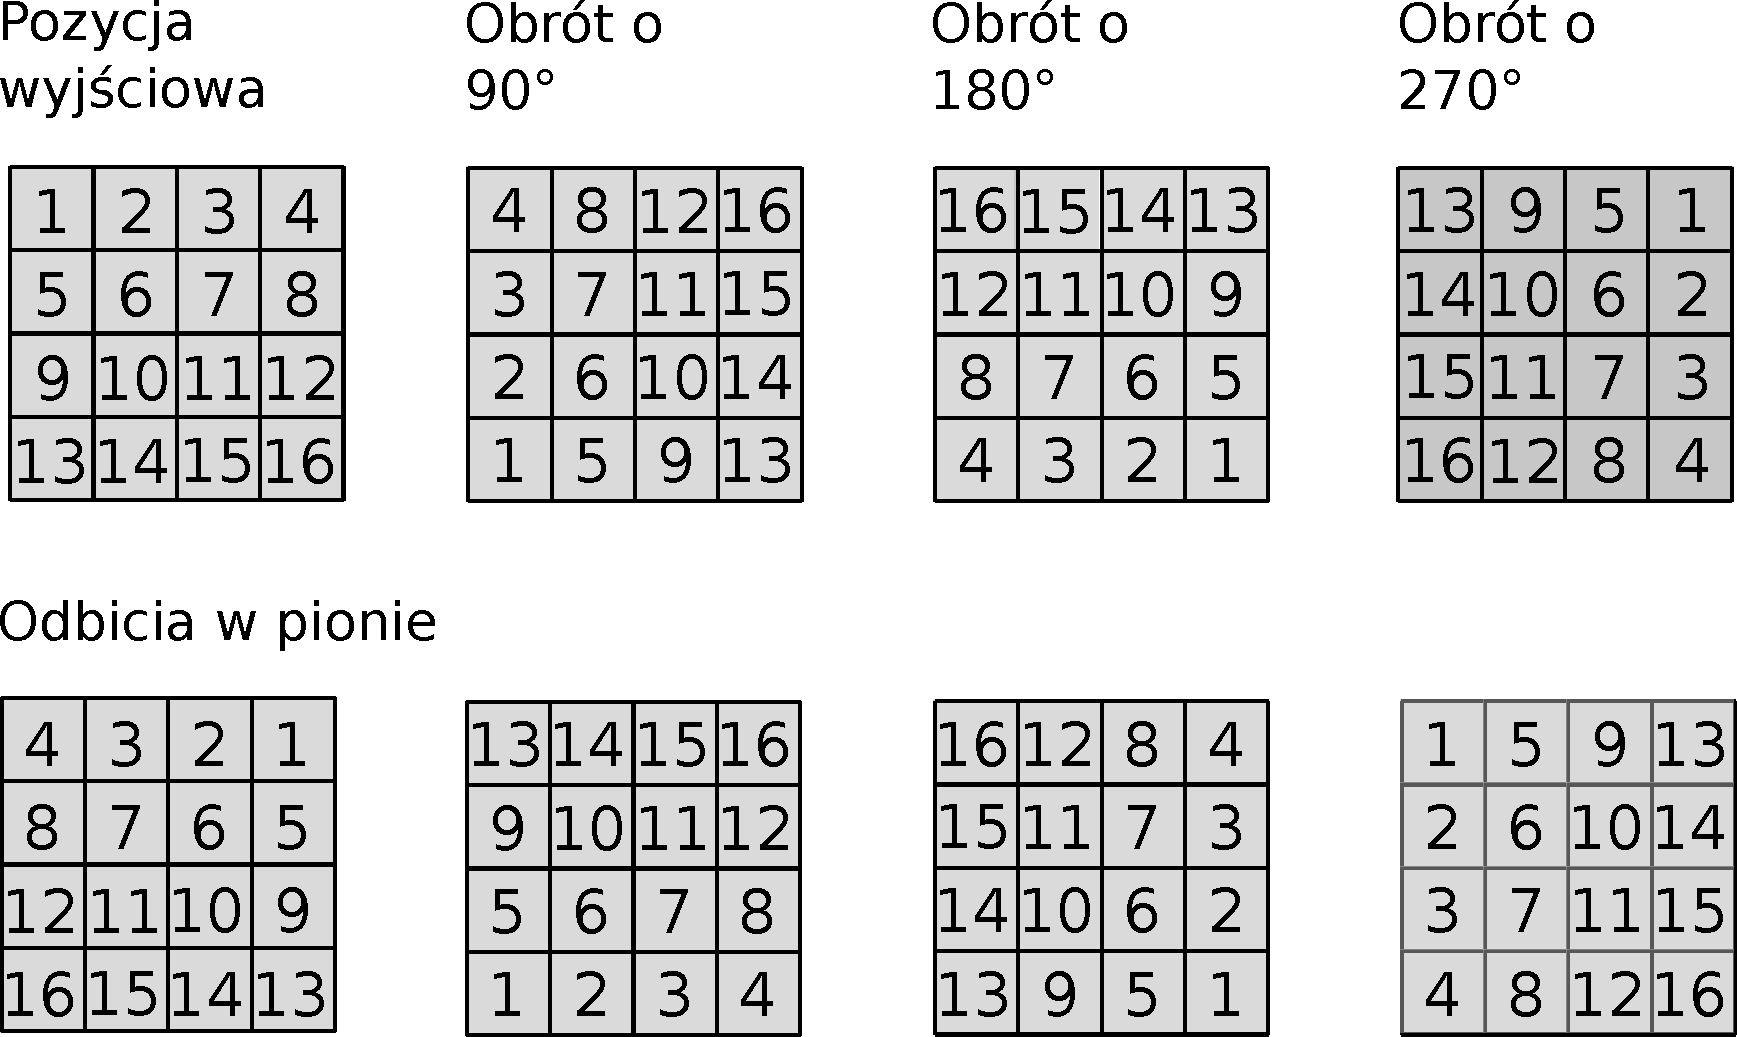
\includegraphics[width=\textwidth]{data/field_order2.pdf}
  \caption{Transformacje planszy nie zmieniające stanu gry}
  \label{fig:field_order2}
\end{figure}


\subsubsection{Przykład}

Rozważmy stan gry przedstawiony na rysunku \ref{fig:exaple_state}.

\begin{figure}[h!]
  \centering
  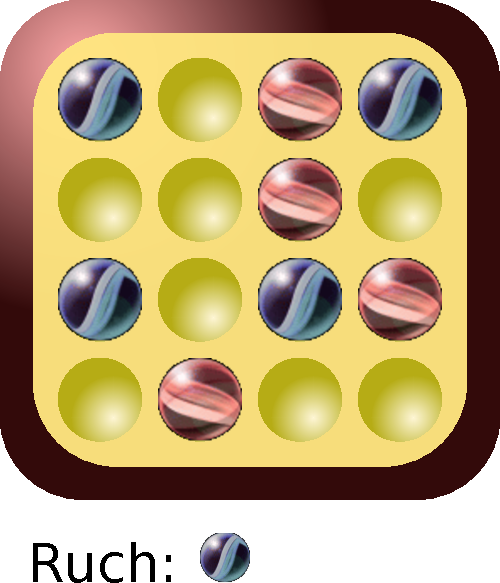
\includegraphics[width=5cm]{data/example_board.pdf}
  \caption{Przykładowy stan gry}
  \label{fig:example_state}
\end{figure}


\subsection{Generacja ruchów dopuszczalnych}

\subsection{Metody przeszukiwania stanów gry}

\subsection{Funkcja oceny heurystycznej stanu gry}

\section{Testy wydajnościowe i porównania algorytmów}

\section{Wnioski}

\begin{thebibliography}{9}

\bibitem{drongowski08_g} Paul J. Drongowski,
  \emph{Basic Performance Measurements for AMD Athlon 64, 
AMD Opteron and AMD Phenom Processors}, Advanced Micro Devices, Inc.,
  2008

\bibitem{drongowski08_ca} Paul J. Drongowski,
  \emph{An introduction to analysis and optimization 
with AMD CodeAnalyst Performance Analyzer}, Advanced Micro Devices, Inc.,
  2008

\end{thebibliography}

\end{document}
